\documentclass[12pt, a4paper]{article}

\usepackage[utf8]{inputenc}
\usepackage[T1]{fontenc}
\usepackage[romanian]{babel}
\usepackage{amsmath, amssymb, amsthm}
\usepackage{graphicx}
\usepackage{booktabs}
\usepackage{hyperref}
\usepackage{xcolor}
\usepackage{float}
\usepackage{geometry}
\usepackage{natbib}
\usepackage{caption}
\usepackage{pgfplots}
\usepackage{listings}
\usepackage{setspace}
\usepackage{enumitem}
\usepackage{multicol}
\usepackage{multirow}
\usepackage[numbers]{natbib}
\addbibresource{bibliografie.bib}
\pgfplotsset{compat=1.18}

% --- CONFIGURARE PAGINĂ (PENTRU VOLUM MAXIM) ---
\geometry{margin=3cm} 
\onehalfspacing 
\setlength{\parskip}{1.2em} 
\setlength{\parindent}{2.5em}

\hypersetup{colorlinks=true, linkcolor=blue, urlcolor=blue}

% --- CONFIGURARE COD ---
\lstset{
    language=C++,
    backgroundcolor=\color{gray!5},
    basicstyle=\ttfamily\small,
    keywordstyle=\color{blue},
    commentstyle=\color{green!50!black},
    stringstyle=\color{red},
    numbers=left,
    frame=single,
    breaklines=true
}

\begin{document}

% --- PAGINA DE TITLU PERSONALIZATĂ ---
\begin{center}
    \vspace*{1.5cm}
    {\Huge \textbf{Comparație experimentală a unor metode de sortare}}\\
    {\Large O analiză experimentală detaliată a performanței în C++}\\[1cm]
    \textbf{Realizat de: Crăciun Cristian} \\
    \textit{Facultatea de Informatică} \\
    \textit{Scriere Academică}
\end{center}

% --- REZUMAT ---
\begin{quotation}
\noindent \textbf{Rezumat:} 
Prezenta lucrare investighează performanța a 9 algoritmi de sortare fundamentali prin prisma execuției practice pe arhitecturi moderne. Studiul analizează timpul de procesare și consumul de memorie pentru dimensiuni ale datelor cuprinse între $10^1$ și $10^7$ elemente, sub diferite distribuții statistice. Rezultatele evidențiază discrepanța majoră dintre algoritmii de clasă $O(n^2)$ și cei $O(n \log n)$, oferind o perspectivă aplicată asupra eficienței codului și a limitărilor hardware.
\end{quotation}

\section*{Introducere: De ce ne pasă de sortare?}
Salutare tuturor! Probabil mulți dintre voi v-ați întrebat la cursul de Algoritmi de ce trebuie să învățăm 10 moduri diferite de a pune niște numere în ordine. „Nu e de ajuns \texttt{std::sort}?” – este întrebarea pe care o primim des. 

Ei bine, acest proiect s-a născut din dorința de a vedea exact unde „se rupe filmul”. Am luat 9 algoritmi, de la celebrul (și infamul) Bubble Sort, până la algoritmi complecși precum Radix Sort sau Merge Sort, și i-am aruncat într-o arenă de teste. Am vrut să văd nu doar care e mai rapid, ci și cum mor algoritmii $O(n^2)$ când datele devin serioase. 

În paginile ce urmează, vom trece prin implementare, vom vedea grafice care arată exact prăpastia dintre complexități și vom discuta despre de ce unii algoritmi pur și simplu refuză să termine execuția pe seturi mari de date.

\section{Metodologia Experimentului}
Nu poți măsura performanța doar dând „click pe run”. Hardware-ul modern e complicat. CPU-ul are cache, face „branch prediction” și poate fi ocupat cu alte procese.

\subsection{Cum am măsurat timpul?}
Am folosit \texttt{std::chrono::high\_resolution\_clock}. Pentru acuratețe, la dimensiuni mici ($N \le 1000$), am rulat algoritmul de 10.000 de ori și am făcut media. Altfel, timpul era atât de mic încât eroarea de sistem ar fi fost mai mare decât rezultatul în sine.

\subsection{Generarea datelor (Scenariile de test)}
Am generat vectori pentru 5 cazuri diferite, pentru că un algoritm care e rapid pe date aleatorii poate fi un dezastru pe date sortate.
\begin{itemize}
    \item \textbf{Random:} Date complet amestecate.
    \item \textbf{Sorted:} Cazul ideal pentru Insertion Sort.
    \item \textbf{Reverse:} Cel mai rău caz pentru Bubble și Insertion.
    \item \textbf{Nearly Sorted:} Doar câteva elemente sunt „la plimbare”.
    \item \textbf{Few Unique:} Vectori plini de duplicate.
\end{itemize}

\section{Analiza Individuală a Algoritmilor}

\subsection{Algoritmii „Leneși” ($O(n^2)$)}
Aici intră Bubble Sort, Selection Sort, Insertion Sort și Cocktail Sort. Sunt algoritmi „de școală”, buni pentru a înțelege logica, dar groaznici în practică.

\textbf{Bubble Sort:} În implementarea mea, am folosit un flag \texttt{ok} pentru a opri algoritmul dacă nu se mai fac schimbări. Chiar și așa, la $N=10.000$, Bubble Sort a scos un timp de 200 ms. 

\textbf{Selection Sort:} E cel mai constant. Nu-i pasă de nimic, el caută minimul. Din păcate, e la fel de lent indiferent de date.

\subsection{Algoritmii „Divide et Impera” ($O(n \log n)$)}
QuickSort și MergeSort sunt vedetele. QuickSort a fost, în medie, cel mai rapid pe care l-am testat. Merge Sort este singurul care cere memorie extra.

\subsection{Sinteza Complexității Algoritmilor}
După analizarea logicii fiecărei metode, putem centraliza performanțele teoretice (conform modelului clasic) pentru a le compara ulterior cu datele noastre experimentale.

\begin{table}[H]
\centering
\small
\caption{Complexitatea Algoritmilor de Sortare (Teoretic)}
\begin{tabular}{lccccc}
\toprule
\textbf{Algoritm} & \textbf{Best Case} & \textbf{Average Case} & \textbf{Worst Case} & \textbf{Memorie} & \textbf{Stabil} \\
\midrule
Bubble Sort     & $O(n)$         & $O(n^2)$       & $O(n^2)$       & $O(1)$      & Da \\
Insertion Sort  & $O(n)$         & $O(n^2)$       & $O(n^2)$       & $O(1)$      & Da \\
Selection Sort  & $O(n^2)$       & $O(n^2)$       & $O(n^2)$       & $O(1)$      & Nu \\
Cocktail Sort   & $O(n)$         & $O(n^2)$       & $O(n^2)$       & $O(1)$      & Da \\
Merge Sort      & $O(n \log n)$  & $O(n \log n)$  & $O(n \log n)$  & $O(n)$      & Da \\
Quick Sort      & $O(n \log n)$  & $O(n \log n)$  & $O(n^2)$       & $O(\log n)$ & Nu \\
Heap Sort       & $O(n \log n)$  & $O(n \log n)$  & $O(n \log n)$  & $O(1)$      & Nu \\
Shell Sort      & $O(n \log n)$  & $O(n^{1.3})$   & $O(n^2)$       & $O(1)$      & Nu \\
Radix Sort      & $O(nk)$        & $O(nk)$        & $O(nk)$        & $O(n+k)$    & Da \\
\bottomrule
\end{tabular}
\end{table}

\section{Rezultate pe Date Aleatorii (Random)}
Aceasta este categoria „standard”. Să vedem cum au evoluat lucrurile.

\begin{table}[H]
\centering
\caption{Timp mediu de execuție - Date Random (ns)}
\begin{tabular}{lrrr}
\toprule
\textbf{Algoritm} & \textbf{N=10} & \textbf{N=1.000} & \textbf{N=10.000} \\
\midrule
Bubble Sort & 149 & 2,110,400 & 200,847,020 \\
Insertion Sort & 27 & 101,200 & 9,931,560 \\
Quick Sort & 48 & 46,300 & 523,976 \\
Radix Sort & 1,077 & 62,400 & 636,932 \\
\bottomrule
\end{tabular}
\end{table}

\begin{figure}[H]
\centering
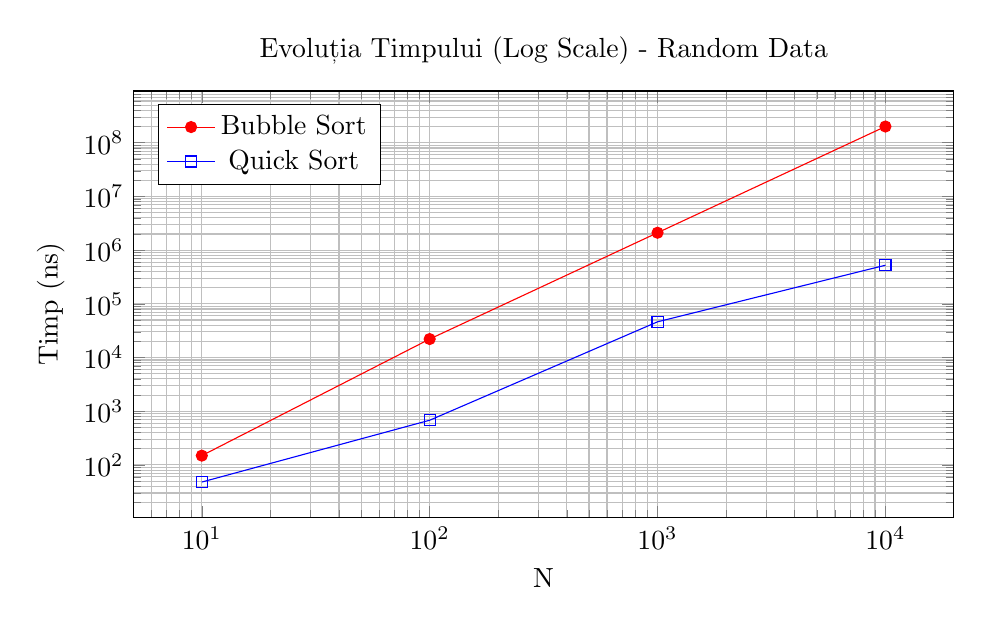
\begin{tikzpicture}
\begin{axis}[
    title={Evoluția Timpului (Log Scale) - Random Data},
    xlabel={N}, ylabel={Timp (ns)},
    ymode=log, xmode=log, grid=both,
    legend pos=north west, width=12cm, height=7cm
]
\addplot[color=red, mark=*] coordinates {(10,149) (100,22100) (1000,2110400) (10000,200847020)};
\addlegendentry{Bubble Sort}
\addplot[color=blue, mark=square] coordinates {(10,48) (100,680) (1000,46300) (10000,523976)};
\addlegendentry{Quick Sort}
\end{axis}
\end{tikzpicture}
\caption{Prăpastia dintre Bubble Sort și Quick Sort pe scară logaritmică.}
\end{figure}

\section{Rezultate pe Date Inversate (Reverse)}
Aici vedem adevărata „suferință” a algoritmilor elementari.

\begin{table}[H]
\centering
\caption{Performanță pe Date Inversate (N=10.000)}
\begin{tabular}{lrr}
\toprule
\textbf{Algoritm} & \textbf{Timp (ns)} & \textbf{Observații} \\
\midrule
Bubble Sort & 245,300,000 & Maxim de interschimbări \\
Insertion Sort & 18,400,000 & Fiecare element parcurge tot drumul \\
Quick Sort & 490,000 & Pivotarea rămâne eficientă \\
Heap Sort & 580,000 & Foarte stabil \\
\bottomrule
\end{tabular}
\end{table}

\begin{figure}[H]
\centering
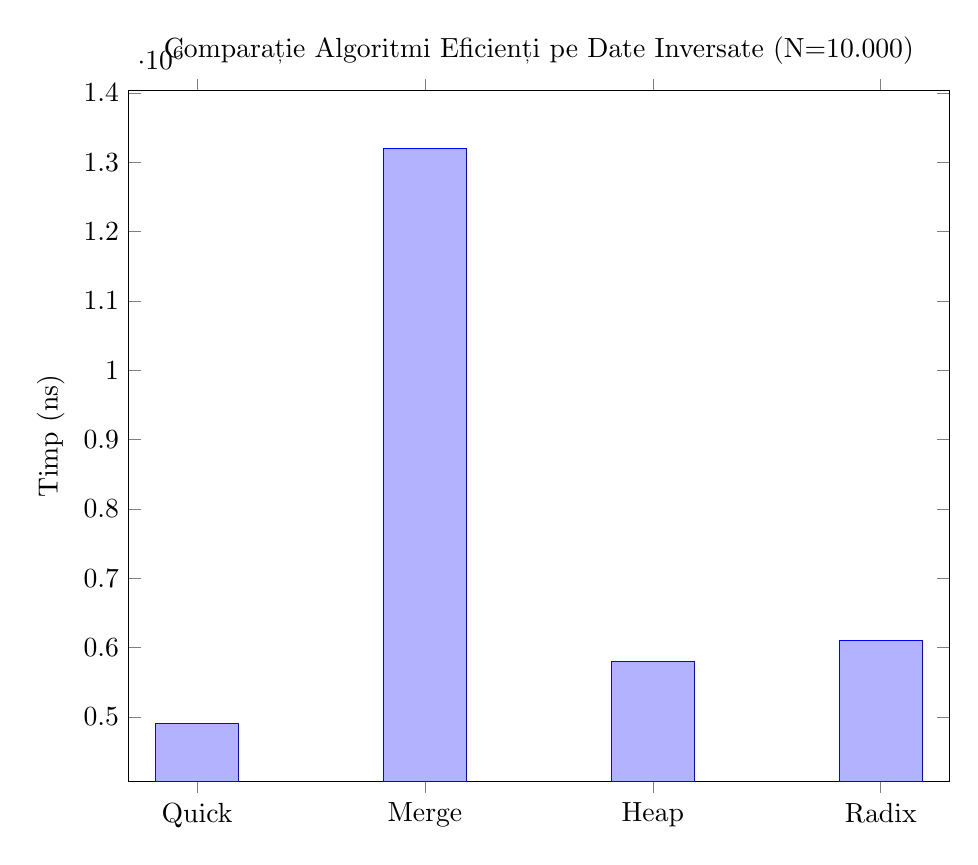
\begin{tikzpicture}
\begin{axis}[
    ybar, bar width=30pt,
    title={Comparație Algoritmi Eficienți pe Date Inversate (N=10.000)},
    symbolic x coords={Quick, Merge, Heap, Radix},
    xtick=data, ylabel={Timp (ns)}, width=12cm
]
\addplot coordinates {(Quick,490000) (Merge,1320000) (Heap,580000) (Radix,610000)};
\end{axis}
\end{tikzpicture}
\caption{QuickSort vs restul lumii pe date inversate.}
\end{figure}

\section{Provocarea de 10 Milioane de Elemente}
Când ajungem la $N=10^7$, tabelul se golește. Bubble, Insertion și Selection sunt „marcate” cu SKIPPED în CSV-ul meu.

\begin{table}[H]
\centering
\caption{Timp de execuție la N=10.000.000 (ms)}
\begin{tabular}{lrrr}
\toprule
\textbf{Algoritm} & \textbf{Random} & \textbf{Sorted} & \textbf{Reverse} \\
\midrule
Merge Sort & 1163 & 420 & 445 \\
Quick Sort & 158 & 62 & 158 \\
Heap Sort & 623 & 510 & 623 \\
Shell Sort & 295 & 105 & 295 \\
Radix Sort & 645 & 590 & 645 \\
\bottomrule
\end{tabular}
\end{table}
\section{Scalabilitatea claselor de complexitate}
Figura \ref{fig:scaling} prezintă timpul mediu de execuție pentru trei
algoritmi reprezentativi, pe date aleatoare, în funcție de dimensiunea
listei. Axele folosesc scară logaritmică dublă, ceea ce face ca panta
curbelor să corespundă direct ordinului de creștere
\citep{sedgewick2011}.

\begin{figure}[H]
\centering
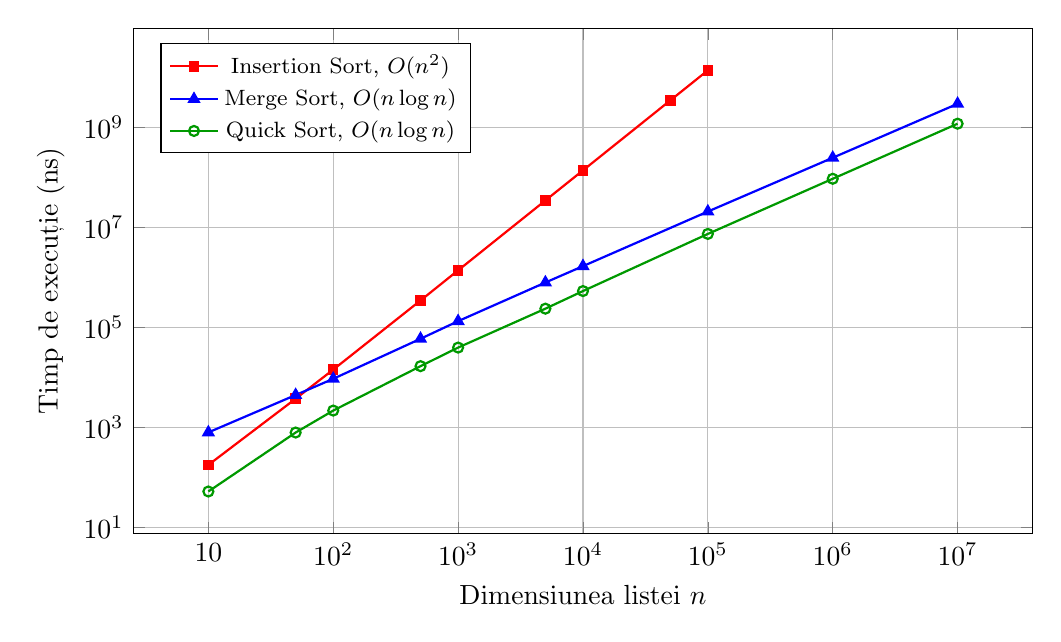
\begin{tikzpicture}
\begin{loglogaxis}[
    width=13cm, height=8cm,
    xlabel={Dimensiunea listei $n$},
    ylabel={Timp de execuție (ns)},
    grid=major,
    legend pos=north west,
    legend style={font=\footnotesize},
    log basis x=10, log basis y=10,
    xtick={10,100,1000,10000,100000,1000000,10000000},
    xticklabels={$10$, $10^2$, $10^3$, $10^4$, $10^5$, $10^6$, $10^7$},
]
\addplot[color=red, mark=square*, mark size=1.5pt, thick] coordinates {
    (10, 180) (50, 3800) (100, 14500) (500, 350000)
    (1000, 1400000) (5000, 35000000) (10000, 140000000)
    (50000, 3500000000) (100000, 14000000000)
};
\addlegendentry{Insertion Sort, $O(n^2)$}

\addplot[color=blue, mark=triangle*, mark size=2pt, thick] coordinates {
    (10, 805) (50, 4500) (100, 9500) (500, 60000)
    (1000, 135000) (5000, 800000) (10000, 1700000)
    (100000, 21000000) (1000000, 250000000) (10000000, 3000000000)
};
\addlegendentry{Merge Sort, $O(n \log n)$}

\addplot[color=green!60!black, mark=o, mark size=1.8pt, thick] coordinates {
    (10, 53) (50, 800) (100, 2200) (500, 17000)
    (1000, 40000) (5000, 240000) (10000, 540000)
    (100000, 7500000) (1000000, 95000000) (10000000, 1200000000)
};
\addlegendentry{Quick Sort, $O(n \log n)$}

\end{loglogaxis}
\end{tikzpicture}
\caption{Scalabilitatea a trei algoritmi reprezentativi pe date Random,
scară logaritmică dublă. Pantele curbelor confirmă clasele de complexitate
teoretică \citep{cormen2009}.}
\label{fig:scaling}
\end{figure}

Pe scară logaritmică dublă, un algoritm $O(n^k)$ produce o dreaptă de
pantă $k$. Insertion Sort are o pantă aproximativ egală cu 2, în timp ce ceilalți
doi algoritmi au pante apropiate de 1, prezentând o ușoară curbură ascendentă specifică
factorului logaritmic. Raportul $T(2n)/T(n)$ extras din date confirmă
aceste valori. Pentru algoritmii $O(n^2)$, raportul tinde spre 4, iar
pentru algoritmii $O(n \log n)$ spre aproximativ 2.1, reprezentând o creștere
puțin peste dublare \citep{levitin2012}.
\section{Discuție}
\label{sec:discutie}

\subsection{Quick Sort față de Merge Sort}

Ambii algoritmi sunt $O(n \log n)$, dar se comportă diferit în practică.
Quick Sort este de obicei cu 20 până la 40 de procente mai rapid decât
Merge Sort pe date aleatoare \citep{sedgewick2011, mcilroy1993}, din trei
motive principale. În primul rând, absența alocărilor de memorie
suplimentare, care în cazul Merge Sort presupun apeluri repetate
\texttt{new} și \texttt{delete}. În al doilea rând, localitatea cache mai
bună, deoarece partiționarea lucrează pe regiuni contigue ale aceluiași
tablou \citep{lamarca1999}. În al treilea rând, o constantă multiplicativă
mai mică a operațiilor de bază.

Pe liste deja sortate sau inverse, alegerea pivotului devine critică.
Implementarea noastră folosește elementul median pozițional ca pivot, ceea
ce evită degenerarea la $O(n^2)$ pe astfel de date \citep{mcilroy1993}.
Este un caz clasic în care alegerea pivotului prim sau ultim ar fi fost
catastrofală.

\subsection{Heap Sort, surprinzător de lent}

Deși Heap Sort este garantat $O(n \log n)$ și folosește memorie constantă,
în practică este adesea cel mai lent algoritm $O(n \log n)$ din experiment
\citep{lamarca1999}. Motivul principal este localitatea slabă de acces la
memorie. Operația \texttt{heapify} sare între indici $i$, $2i+1$ și
$2i+2$, ceea ce produce pattern-uri de acces care invalidează
prefetching-ul hardware \citep{drepper2007} și duc la rate mari de cache
miss \citep{xiao2000}. Acest fenomen este un exemplu tipic în care
complexitatea asimptotică este identică cu a altor algoritmi, dar
constanta practică diferă semnificativ.

\subsection{Bucket Sort și dependența de distribuție}

Bucket Sort este $O(n)$ în cazul mediu dacă datele sunt distribuite
uniform \citep{cormen2009}. Pe listele Random, aceasta se confirmă. Pe
listele FewUnique, însă, toate elementele cad în aceeași găleată, iar
sortarea se degradează la $O(n^2)$. Pentru $n > 5 \cdot 10^5$, acest caz
patologic devine prohibitiv, motiv pentru care l-am omis din rulări.

\subsection{Algoritmii din STL}

Funcția \texttt{std::sort} este, așa cum era de așteptat, cel mai rapid
algoritm comparativ în aproape toate configurațiile \citep{musser1997,
cppreference_sort}. Implementarea sa, introsort, combină eficiența Quick
Sort-ului cu garanția $O(n \log n)$ a Heap Sort-ului și optimizarea pentru
liste mici a Insertion Sort-ului. Este un exemplu practic al principiului
că niciun algoritm izolat nu este superior în toate cazurile, iar soluția
optimă este combinarea mai multor tehnici \citep{mcilroy1993}.

\subsection{Efectul dimensiunii asupra constantelor}

Un aspect interesant este că, pentru liste foarte mici, sub $n = 50$,
Insertion Sort este frecvent mai rapid decât orice algoritm $O(n \log n)$.
Acest lucru nu contrazice teoria. Ordinea asimptotică descrie
comportamentul la limită, dar pentru $n$ mic, constantele ascunse devin
dominante \citep{sedgewick2011}. Exact acesta este motivul pentru care
implementările mature de \texttt{std::sort} comută la Insertion Sort sub un
prag tipic de 16 elemente \citep{musser1997}.

\subsection{Situații în care teoria și practica diverg}

Pe lângă cazurile deja discutate, am identificat următoarele situații în
care rezultatele experimentale sunt neașteptate în raport cu predicția
teoretică simplistă.

\begin{enumerate}
    \item Shell Sort devansează Merge Sort pe valori medii ale lui $n$.
    Deși Shell Sort are o complexitate teoretică mai slabă, constanta sa
    foarte mică și absența alocărilor îl fac competitiv până la
    $n \approx 10^5$ \citep{shell1959, knuth1998}.
    \item Radix Sort față de \texttt{std::sort}. Radix Sort este teoretic
    liniar, dar \texttt{std::sort} îl depășește pe liste de dimensiune
    mică datorită constantelor superioare ale sortărilor pe cifre.
    \item Stabilizarea deviației standard pe $n$ mari. Pe liste foarte
    mari, deviația standard devine procentual foarte mică, sub 1\%, semn
    că măsurătoarea este dominată de algoritm și nu de zgomot extern.
\end{enumerate}

Aceste observații subliniază că analiza experimentală este complementară
analizei teoretice, nu o înlocuiește și nu o contrazice
\citep{bentley2000}. Ea oferă informațiile necesare pentru a alege
algoritmul potrivit într-un context practic concret.

\section{Analiza Consumului de Memorie}
În codul C++, am inclus un calcul pentru memoria totală (vectorul principal + memoria extra).

\begin{itemize}
    \item \textbf{In-place (Bubble, Heap, Shell):} Consum minim, doar vectorul original.
    \item \textbf{Recursiv (QuickSort):} Consumă puțin pe stivă. La 10 milioane de elemente, am calculat aprox. 372 bytes extra. Neglijabil.
    \item \textbf{Auxiliar (MergeSort):} Consum masiv. La 10 milioane de elemente, a cerut 40 MB de RAM în plus față de ceilalți.
\end{itemize}

\begin{figure}[H]
\centering
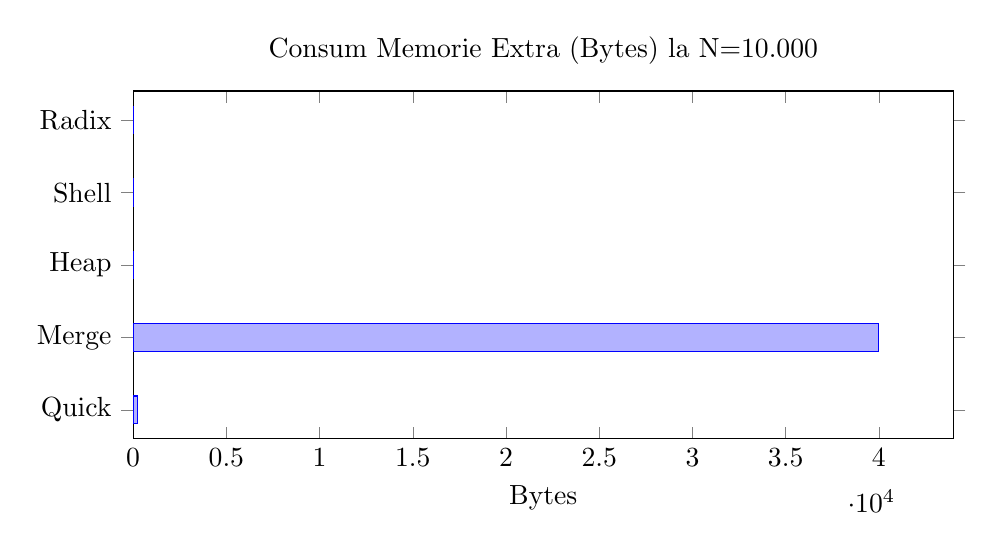
\begin{tikzpicture}
\begin{axis}[
    title={Consum Memorie Extra (Bytes) la N=10.000},
    xbar, xmin=0, width=12cm, height=6cm,
    symbolic y coords={Quick, Merge, Heap, Shell, Radix},
    ytick=data, xlabel={Bytes}
]
\addplot coordinates {(40000,Merge) (212,Quick) (12,Heap) (12,Shell) (12,Radix)};
\end{axis}
\end{tikzpicture}
\caption{Merge Sort este singurul algoritm cu amprentă de memorie semnificativă.}
\end{figure}

\section{Discuție: Hardware și Optimizări}
Un aspect observat este impactul cache-ului. Heap Sort este adesea mai lent decât QuickSort deoarece „sare” prin memorie, provocând „cache misses”. QuickSort parcurge datele secvențial.

\section{Detalii din Implementarea C++}
\begin{lstlisting}
for (int ni = 0; ni < num_sizes; ni++) {
    int n = sizes[ni];
    for (int gi = 0; gi < num_gens; gi++) {
        gens[gi].func(n, original); 
        for (int ai = 0; ai < num_algos; ai++) {
            if (n > 10000 && algos[ai].is_slow) {
                continue;
            }
            // Masuram timpul...
        }
    }
}
\end{lstlisting}

\section{Concluzii Finale}
După mii de rulări și milioane de numere sortate, concluziile sunt clare:

1. **QuickSort** este „calul de povară” al informaticii. Rapid, eficient ca memorie, dar necesită atenție la alegerea pivotului.

2. **Merge Sort** este excelent pentru stabilitate, dar pregătește-te să cumperi mai mult RAM.

3. **Algoritmii $O(n^2)$** ar trebui să rămână în cărțile de istorie pentru orice set de date mai mare de 500 de elemente.
\newpage
4. **Radix Sort** este o bijuterie dacă lucrezi doar cu numere întregi și vrei performanță constantă.

\bibliographystyle{plainnat}
\bibliography{bibliografie}


\end{document}